I gruppi di pannelli sono stati progettati per offrire agli utenti una visione completa e dettagliata di un aspetto specifico della città. Ogni gruppo è composto da una serie di pannelli che collaborano per presentare informazioni relative a una singola categoria di dati, come temperatura, umidità, presenza di polveri sottili e altre metriche pertinenti. 

Questi pannelli sono appositamente configurati per essere interattivi e fornire agli utenti dettagli in risposta alle azioni eseguite.
\\
\subsubsection{City Manager}
Il gruppo di pannelli "City Manager" è stato appositamente concepito per offrire agli utenti una panoramica dettagliata e completa delle informazioni relative alla città. Questo insieme di pannelli è stato progettato con l'obiettivo di fornire una visione esaustiva e immediata dello stato attuale del contesto urbano.\\
Il gruppo è composto da quattro pannelli principali:
\begin{itemize}
    \item \textbf{Pannello di selezione delle celle}: consente agli utenti di selezionare le variabili inerenti alle celle della città affinché il gruppo di pannelli possa visualizzare le informazioni corrispondenti;
    \item \textbf{Mappa dei sensori}: visualizza la posizione dei sensori desiderati nella città;
    \item \textbf{Punteggio di salute}: visualizza il punteggio di salute della città, generato dal calcolo di un indice di qualità delle misurazioni effettuate dai sensori;
    \item \textbf{Lista delle avvertenze}: visualizza le avvertenze relative alla città. Queste avvertenze sono generate dal sistema in base alle misurazioni effettuate dai sensori e sono visualizzate in tempo reale.
\end{itemize}
\begin{figure}[H]
    \centering
    \fbox{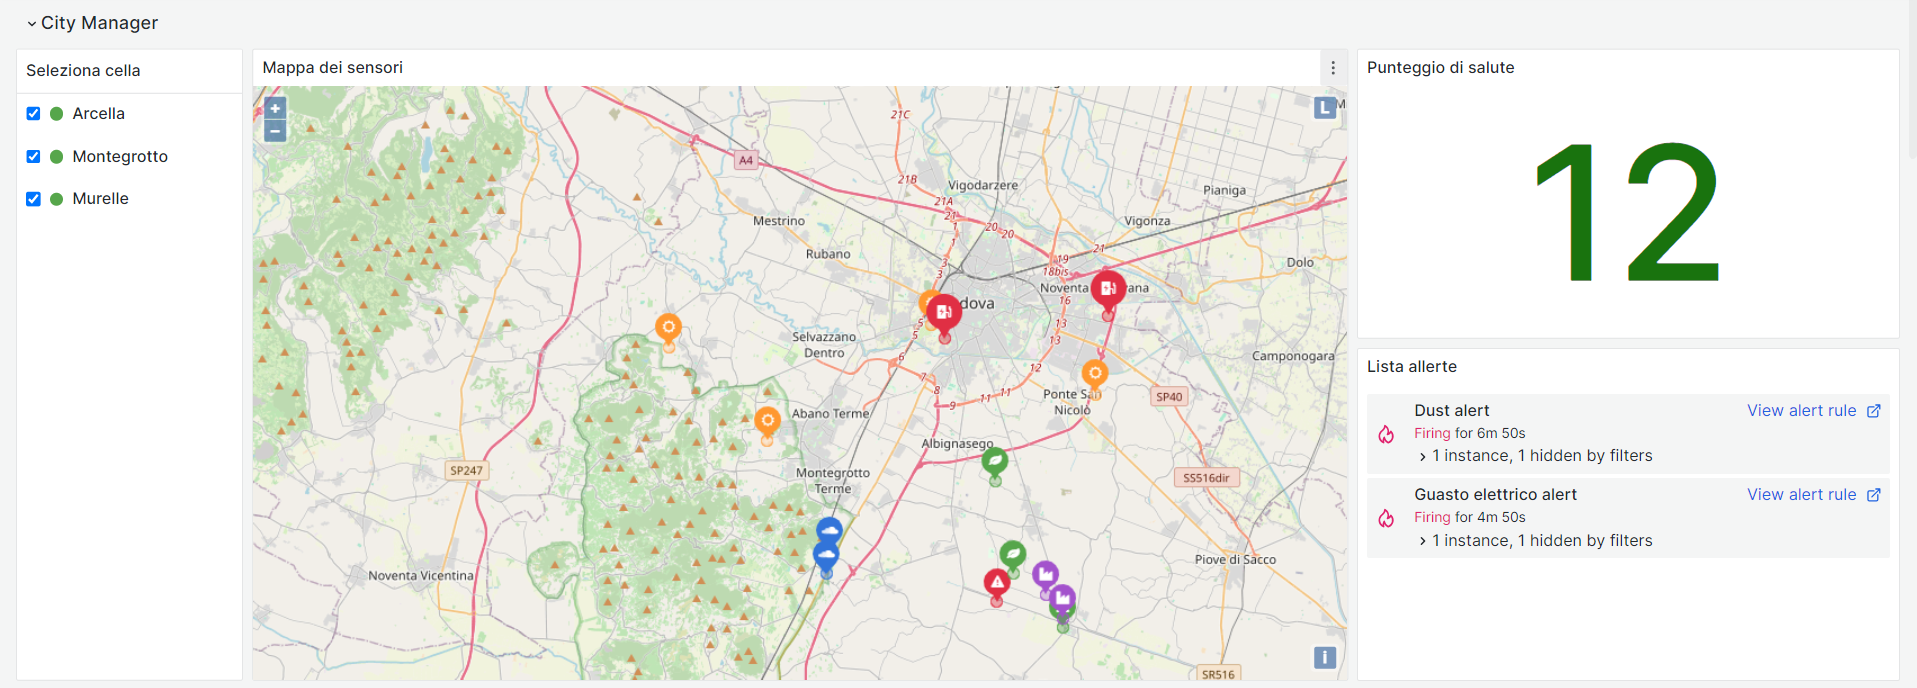
\includegraphics[width=15cm]{../Images/ManualeUtente/Light/gruppo_pannelli_city_manager.png}}
    \caption{Gruppo di pannelli "City Manager"}
    \label{fig:my_label}
\end{figure}


\subsubsection{Temperatura, Umidità, Polveri sottili}
I gruppi di pannelli "Temperatura", "Umidità" e "Polveri sottili" hanno una struttura simile. Per facilità di comprensione, verrà descritto solo il gruppo di pannelli "Temperatura" ma le stesse informazioni si applicano anche agli altri due gruppi.\\ 
Il gruppo di pannelli "Temperatura" è composto da tre pannelli:
\begin{itemize}
    \item \textbf{Pannello di selezione dei sensori}: consente agli utenti di selezionare i sensori desiderati affinché il gruppo di pannelli possa visualizzare le informazioni corrispondenti;
    \item \textbf{Grafico a linee}: visualizza la temperatura rilevata dai sensori selezionati tramite un grafico a linee descritto nel paragrafo  ~\hyperlink{par:grafico_linee}{\S 3.2.3 - Grafico a linee};
    \item \textbf{Temperatura media}: visualizza la temperatura media rilevata dai sensori selezionati in un determinato intervallo di tempo. La temperatura media viene mostrata all'utente attraverso un grafico "visualizzazione statistiche" come descritto nel paragrafo ~\hyperlink{par:visu_stat}{\S 3.2.3 - Grafico visualizzazione statistiche} e attraverso un valore numerico.
\end{itemize}
\begin{figure}[H]
    \centering
    \fbox{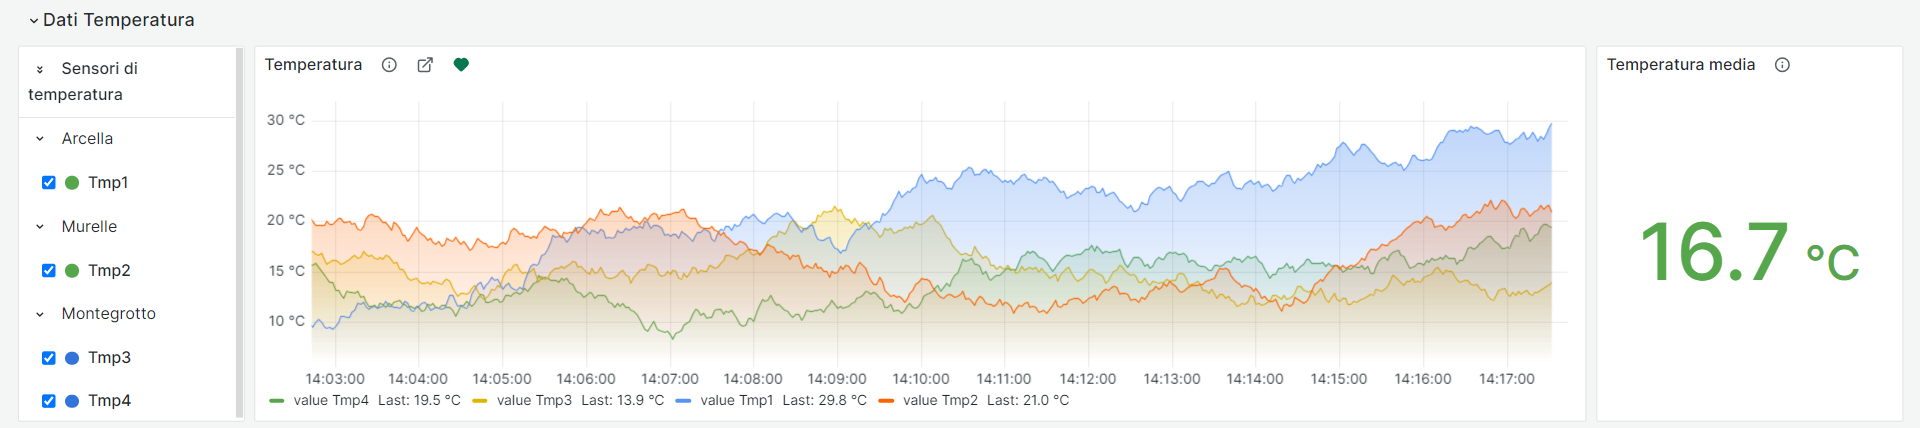
\includegraphics[width=15cm]{../Images/ManualeUtente/Light/gruppo_pannelli_temperatura.png}}
    \caption{Gruppo di pannelli "Temperatura"}
    \label{fig:my_label}
\end{figure}

\subsubsection{Isole ecologiche}
Il gruppo di pannelli "Isole ecologiche" è stato progettato per fornire una visione completa delle informazioni relative alle isole ecologiche.\\
Questo gruppo di pannelli differisce dagli altri descritti sopra in quanto al posto della visualizzazione della temperatura media è presente un grafico a quadrante come descritto nel paragrafo ~\hyperlink{par:grafico_quadrante}{\S 3.2.3 - Grafico a quadrante} che visualizza la percentuale di riempimento delle isole ecologiche.\\
\begin{figure}[H]
    \centering
    \fbox{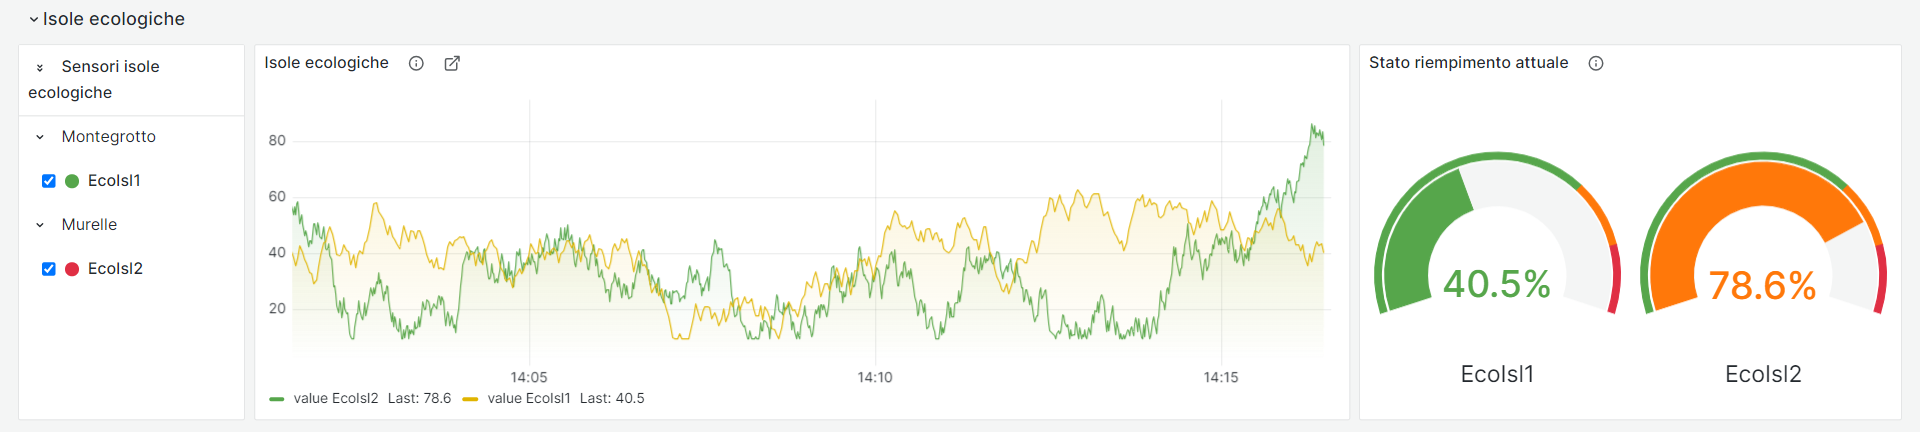
\includegraphics[width=15cm]{../Images/ManualeUtente/Light/gruppo_pannelli_isole.png}}
    \caption{Gruppo di pannelli "Isole ecologiche"}
    \label{fig:my_label}
\end{figure}


\subsubsection{Presenza acqua, Colonnine di ricarica, Guasti elettrici}
I gruppi di pannelli "Presenza acqua", "Colonnine di ricarica" e "Guasti elettrici" hanno una struttura simile. Per facilità di comprensione, verrà descritto solo il gruppo di pannelli "Presenza acqua" ma le stesse informazioni si applicano anche agli altri due gruppi.\\
Il gruppo "Presenza acqua" è composto da quattro pannelli:
\begin{itemize}
    \item \textbf{Sensori presenza acqua}: consente agli utenti di selezionare le variabili (descritte in dettaglio nella sezione ~\hyperlink{par:gestione_variabili_panel}{\S3.2.4}) relative ai sensori desiderati affinché il gruppo di pannelli possa visualizzare le informazioni corrispondenti;
    \item \textbf{Sensori di soglia non attivi}: visualizza i sensori di soglia non attivi tramite un pannello di tipo "visualizzazione statistiche" come descritto nel paragrafo ~\hyperlink{par:visu_stat}{\S 3.2.3 - Grafico visualizzazione statistiche};
    \item \textbf{Sensori di soglia attivi}: visualizza i sensori di soglia attivi tramite un pannello di tipo "visualizzazione statistiche" come descritto nel paragrafo ~\hyperlink{par:visu_stat}{\S 3.2.3 - Grafico visualizzazione statistiche};
    \item \textbf{Sensori di livello acqua}: visualizza i sensori di livello dell'acqua in tabella tramite un pannello di tipo "vista tabellare" come descritto nel paragrafo ~\hyperlink{par:tabella}{\S3.2.3 - Vista tabellare}.
\end{itemize}
\begin{figure}[H]
    \centering
    \fbox{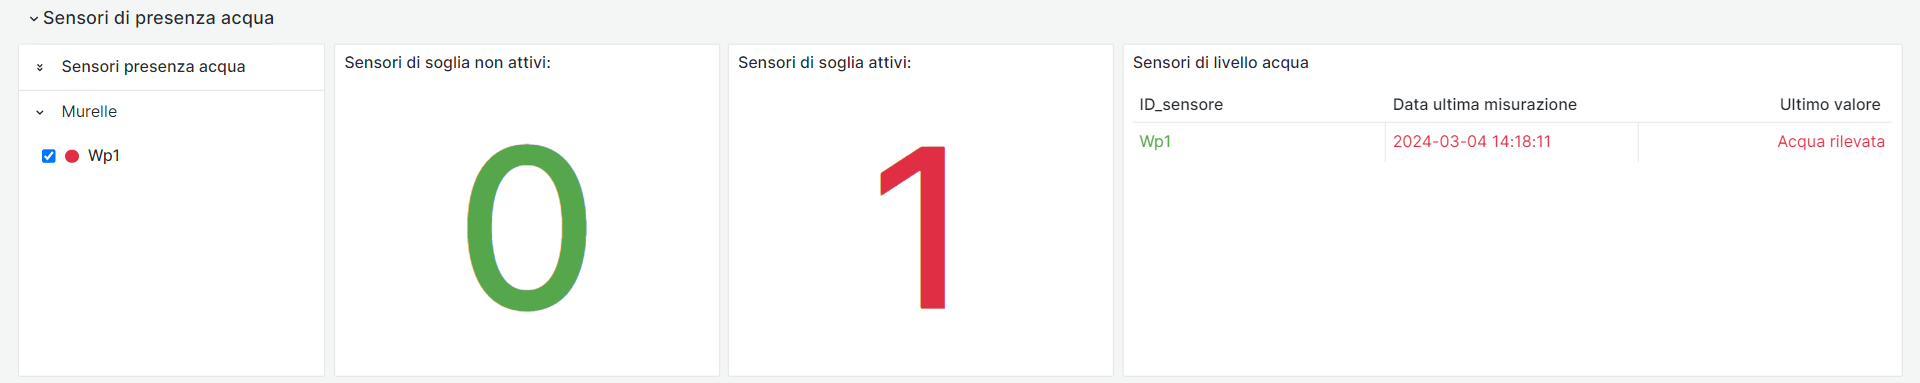
\includegraphics[width=15cm]{../Images/ManualeUtente/Light/gruppo_pannelli_presenza_acqua.png}}
    \caption{Gruppo di pannelli "Presenza acqua"}
    \label{fig:my_label}
\end{figure}

\subsubsection{Minimizzare e massimizzare i gruppi di pannelli}
Ogni gruppo di pannelli può essere minimizzato o massimizzato. Per minimizzare un gruppo di pannelli, l'utente deve fare clic sul nome del gruppo di pannelli o sulla freccetta posta vicino a esso. Per tornare alla visualizzazione massimizzata, l'utente deve fare nuovamente clic sul nome del gruppo di pannelli o sulla freccetta.\\
\begin{figure}[H]
    \centering
    \fbox{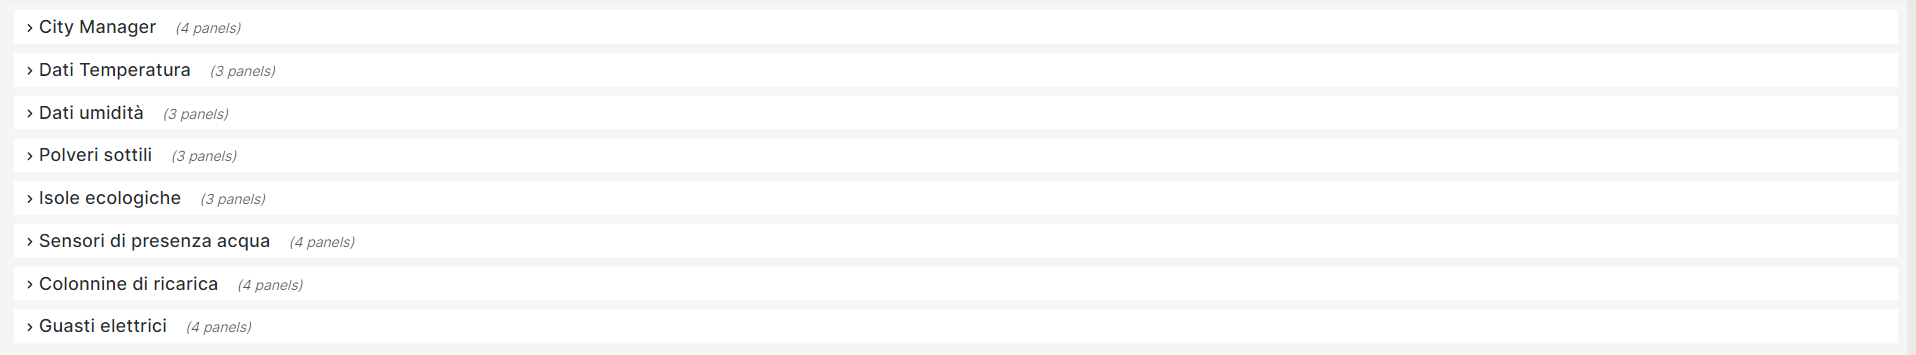
\includegraphics[width=13cm]{../Images/ManualeUtente/Light/gruppo_pannelli_chiusi.png}}
    \caption{Gruppo di pannelli minimizzati}
    \label{fig:my_label}
\end{figure}